\section{Software requirements specification}\label{sec:srs}

\subsection{Problem domain and purpose of our system}\label{ssec:intro}
As mentioned earlier sleep deprivation is a prevalent problem that society faces.
When constructing the application we wanted it to be accessible to the general public as it was identified earlier that sleep deprivation has the potential to affect everyone.
It was identified that the main functionality of our system would be to aid users to track and compare their sleep through the Neuromind headset.

\subsection{Stakeholders involved and the elicitation process:}\label{ssec:stakeholders}
In order to elicit requirements, a questionnaire was constructed. Majority of the stakeholders involved were flight attendants from United Airlines.
In order to get a more diverse range of views to accomodate for diversity, an interview was conducted on a university student with a part time job.
Responses from participants validated our specific problem by justification both in the questionnaire and in the interviews.
We also constructed new requirements from group meetings through the agile process as group members working with specific requirements
identified that requirements could be refined to accomodate for a broader usage.

\subsection{How conflicts between requirements were managed:}\label{ssec:conflicts}
Throughout the course of the project, requirements were refined when group
meetings were conducted and observations by the group were made.
In particular, our team noticed that in order for the system to successfully calculate sleep cycle data,
it had to be extracted from the data calculated by the headset.

Another major requirement that was refined was the client interface.
This initially did not have any sub-requirements, but later sub-requirements had to be added in order for the stakeholder to be able to view processed data.
Without continuous communications between group members and stakeholder contact these optimisations would not have been possible.

Furthermore, towards the end of our project the client requirement remained, but another functional
requirement that we wanted to integrate into our software was the Graphical User Interface (GUI).
It had been expressed in the questionnaire that a graph to view sleep cycle data would be desirable for the end user.
Just having a Graphical user interface independent of the other functionalities would segment our system,
so as a group we devised to incorporate the GUI into our framework to ensure that it would be easier for
the user to interact with the system whilst maintaining a cohesive system.

\subsection{UseCase Diagram:}\label{ssec:UCD}
\begin{figure}[H]
  \centering
  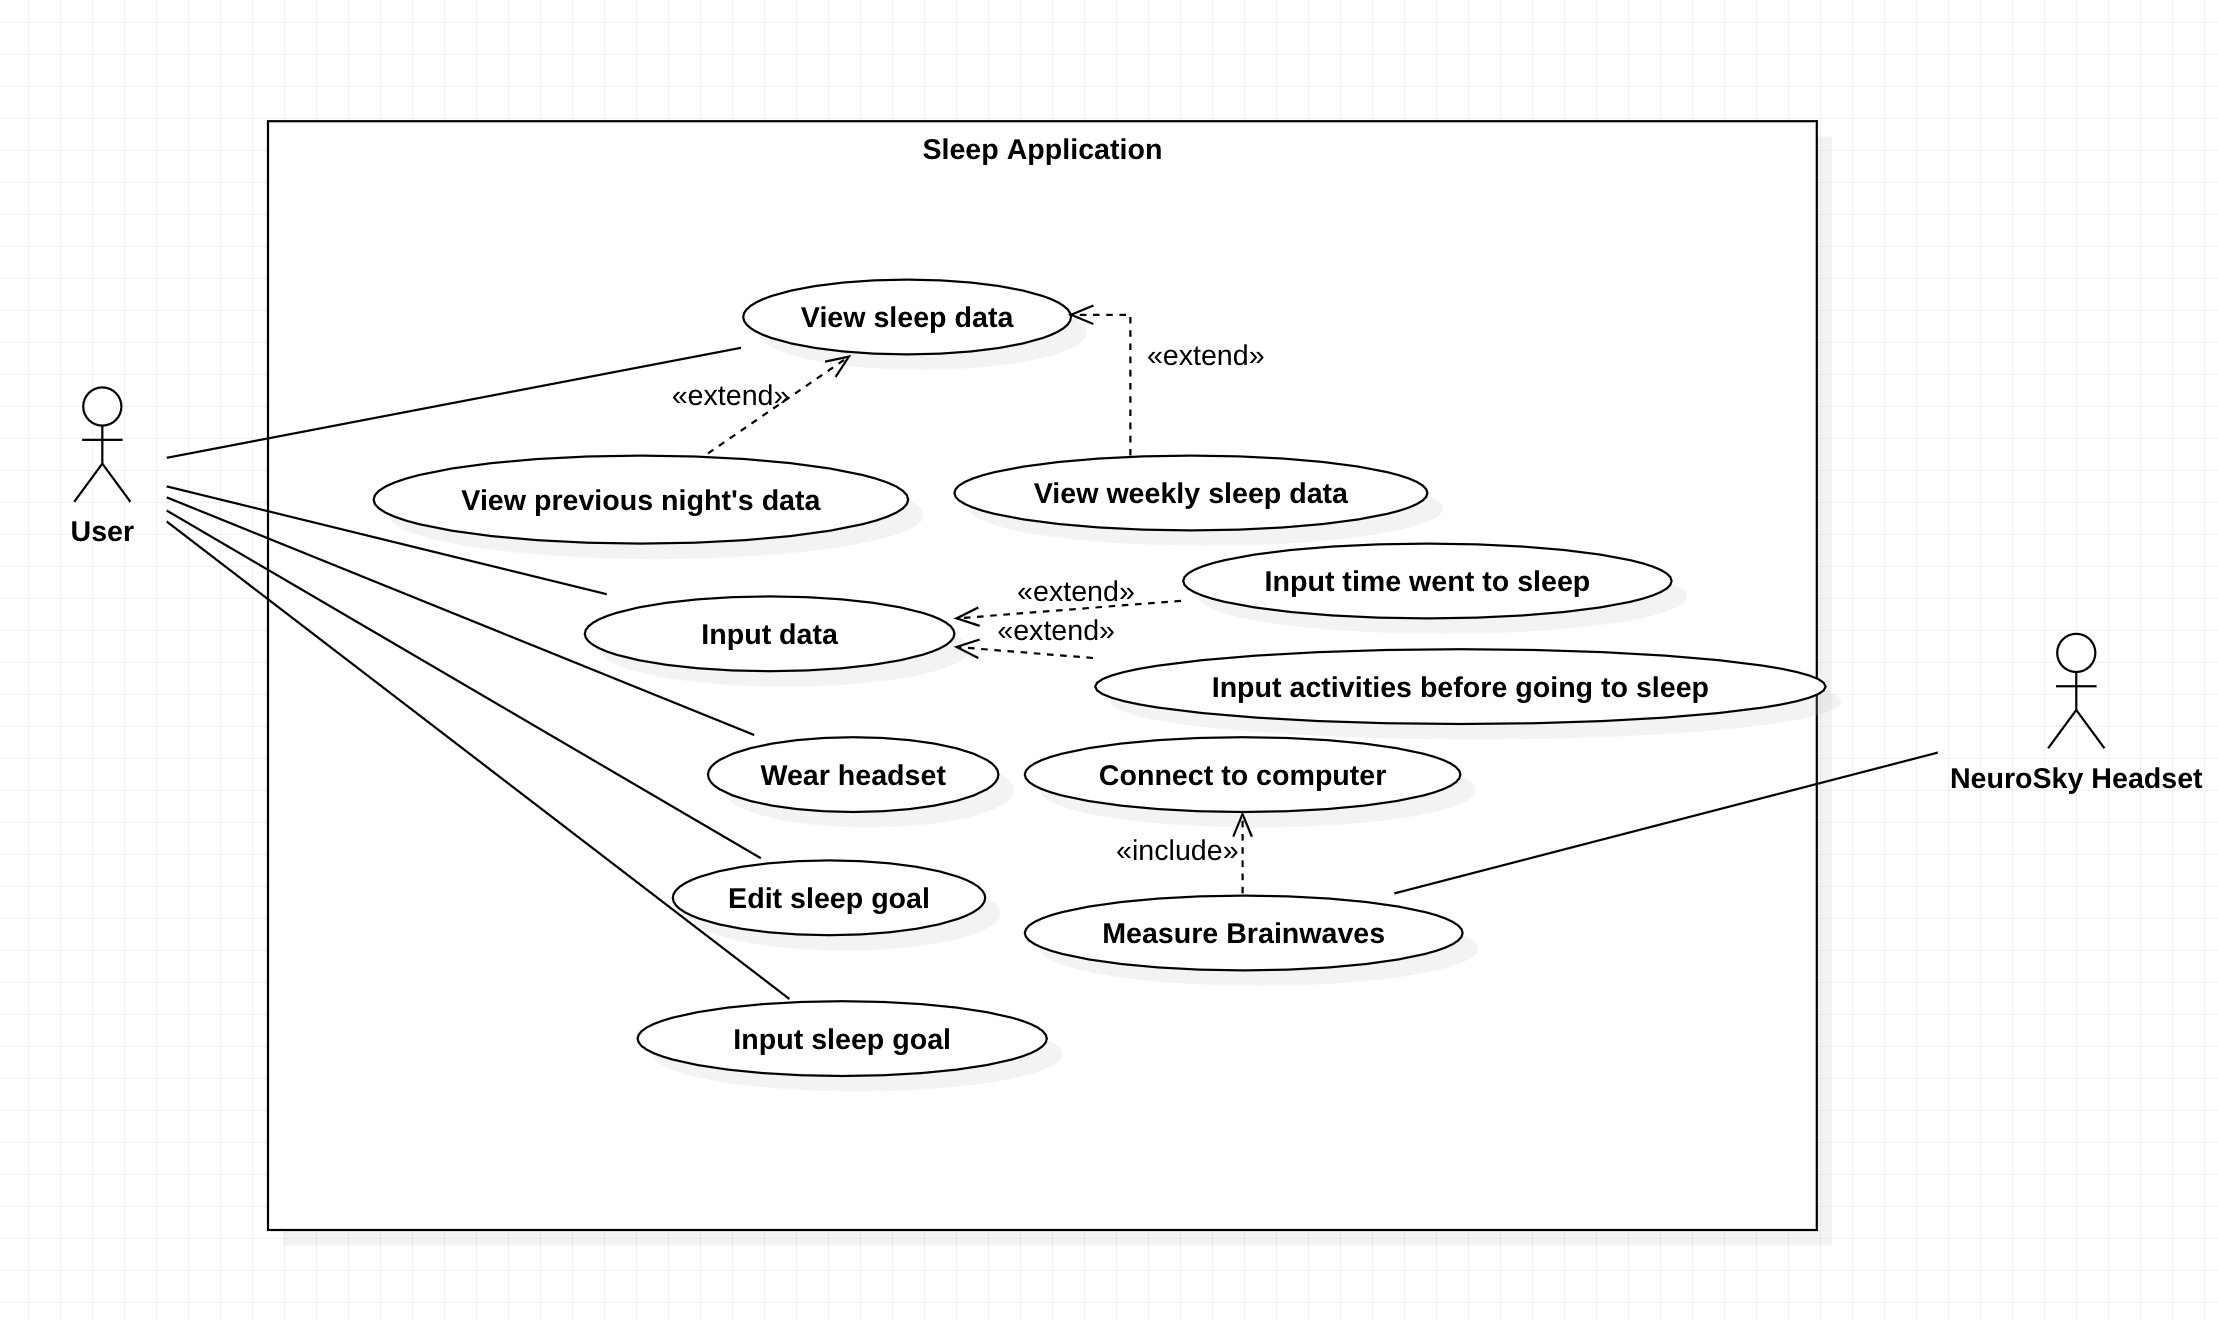
\includegraphics[width=1\textwidth]{UseCaseDiagram}
  \caption{Use Case Diagram}\label{img:use-case-diagram}
\end{figure}
Semantics:
The headset is the external hardware which the user has to wear in order to get a recording.
Once the user is wearing the headset, it can connect to the computer and then measure the user’s brainwaves.
The user is the general audience who will interact with our system.
The user can view sleep data they have inputted into the system using the headset.
They can view either their previous night’s data or last weeks data.
They can also set personal sleep goals which will allow them to then manage their goals that will be saved in the system.
They can also input the time they have previously went to sleep on nights they did not wear the headset.

\subsection{Scenarios:}\label{ssec:scenar}
\subsubsection{Scenario 1:}\label{ssec:scenar1}
Scenario 1:
Actor: User of the system
Goal: Measuring sleep data
Pre conditions:
  1. The user has neurosky headset
  2. The user has thinkgear socket connector installed on their laptop
  3. The user has our application installed.
\begin{figure}[H]
  \centering
  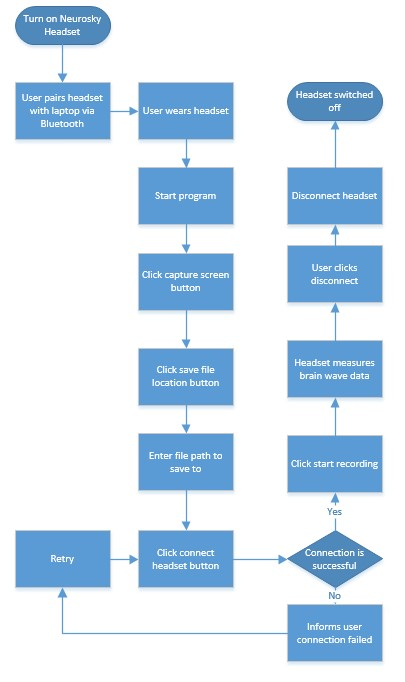
\includegraphics[width=0.5\textwidth]{UseCaseScenario1}
  \caption{Scenario 1}\label{img:usecasescenario1}
\end{figure}

\subsubsection{Scenario 2:}\label{ssec:scenar2}
Scenario 2:
Actor: The user of the system
Goal: View line graph of  brain activity throughout the time the headset was worn.
Preconditions:
The user has the application installed.
Scenario 1 has been completed at least once.
The user has already opened the application.
\begin{figure}[H]
  \centering
  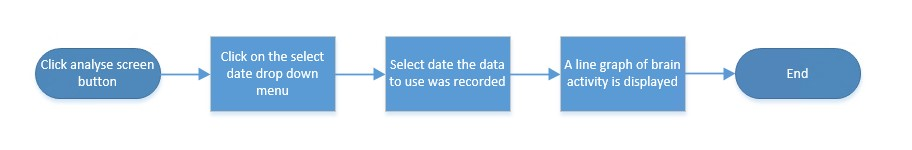
\includegraphics[width=1\textwidth]{UseCaseScenario2}
  \caption{Scenario 2}\label{img:usecasescenario2}
\end{figure}

\subsection{Non-Functional Requirements}\label{ssec:non-functional-requirements}

\renewcommand*{\arraystretch}{1.4}
\begin{requirements}
  \reqsec{soft-devel}  
    \req{agile-scrum}
    \req{3-sprints}
    \req{1-3-weeks}
    \req{review-reqs}
    \req{risk-management}

  \reqsec{expanding-initial}
    \req{expand-non-func}
    \req{expand-func}
    \req{additional-reqs}

  \reqsec{background-research}
    \req{4-articles}
    \req{8-articles}
    \req{8-articles}
    \req{8-articles}
    \req{core-peer-reviewed}
    \req{additional-web}
    \req{classify-rem-cycles}

  \reqsec{ethical-issues}
    \req{ethical-issues}

  \reqsec{testing}
    \req{test-driven-approach}
    \req{evidence-testing}
    \req{state-hypothesis}
    \req{valid-analysis}
\end{requirements}

\subsection{Functional Requirements}\label{ssec:functional-requirements}

\begin{requirements}
  \reqsec{viewing-collecting-data}
    \req{interface-headset}
    \subreq{connect-headset}
    \subreq{disconnect-headset}
    \subreq{read-data-headset}
    \req{store-data}
    \subreq{facilitate-saving}
    \subreq{facilitate-conversion}
    \req{extract-data}
    \subreq{extract-attention-meditation}
    \subreq{calculate-moving-average}
    \subreq{extract-sleep-percentage}
    \subreq{extract-sleep-time}
    \req{present-data}
    \subreq{present-data-table}
    \subreq{present-hypnogram}
    \req{manual-entry}
    \req{apply-sorting-algorithm}
    \req{implement-cli}
    \subreq{allow-user-record-data}
    \subreq{specify-time-record}
    \subreq{allow-user-change-format}
    \subreq{allow-user-extract-calculate}
    \subreq{cli-process-sleep-data}
    \subreq{cli-sort-display}
    \req{GUI-requiremnt}
    \subreq{allow-GUIuser-connect-disconnect}
    \subreq{allow-GUIuser-record-data}
    \subreq{GUIallow-user-change-format}
    \subreq{GUIallow-playback-Data}
    \subreq{GUI-process-sleep-data}
    \subreq{GUI-sort-display}
    \subreq{GUI-viewGraph}

  \reqsec{identifying-trends-data}
    \req{compare-sleep-data}

  \reqsec{goals-achievements}
    \req{allow-manage-goals}
    \req{permit-set-goal}
    \req{update-change-goal}
    \req{motivate-user}

  \reqsec{manage-data-periodically}
    \req{delete-data}
\end{requirements}
